\chapter{Grupos cocientes y Teoremas de isomorfía}
Este tema se centrará en las relaciones de equivalencia $\prescript{}{H}{\sim}$ y $\sim_H$ definidas en el capítulo anterior, donde ya vimos propiedades de estas relaciones (recordamos la Proposición~\ref{prop:biyecciones_conj_cocientes}), como que $G/\prescript{}{H}{\sim}$ y $G/\sim_H$ eran biyectivos o el Teorema de Lagrange. Estaremos especialmente interesados en el caso de que los conjuntos cocientes de estas dos relaciones de equivalencia coincidan, propiedad que nos dará los Teoremas de Isomorfía, que son el principal objeto de estudio de este tema.

\begin{definicion}[Subgrupos normales]
    Sea $G$ un grupo y $H<G$, diremos que $H$ es un subgrupo normal de $G$, denotado por $H \lhd G$, si las clases laterales de cada elemento coinciden, es decir, si:
    \begin{equation*}
        xH = Hx \qquad \forall x\in G
    \end{equation*}
    En cuyo caso, tendremos que $G/\prescript{}{H}{\sim\ } = G/\sim_H$, y notaremos a este conjunto como $G/H$, al llamaremos \underline{conjunto de las clases laterales de $H$ en $G$}. 
\end{definicion}

\begin{definicion}[Conjugado]
    Sea $G$ un grupo, $H\subseteq G$ y $x\in G$, definimos el conjugado de $H$ por $x$ como el conjunto:
    \begin{equation*}
        xHx^{-1} = \{xhx^{-1} \mid h\in H\}
    \end{equation*}
\end{definicion}

\begin{prop}
    Sea $G$ un grupo, $H<G$ y $x\in G$, entonces $xHx^{-1}< G$.
    \begin{proof}
        Para ello, sean $xh_1x^{-1}, xh_2x^{-1}\in xHx^{-1}$, entonces:
        \begin{equation*}
            xh_1x^{-1}{(xh_2x^{-1})}^{-1} = xh_1x^{-1}xh_2^{-1}x^{-1} = xh_1h_2^{-1}x^{-1} \in xHx^{-1}
        \end{equation*}
        Ya que como $H$ es un subgrupo de $G$, entonces $h_1h_2^{-1}\in H$.
    \end{proof}
\end{prop}~\\

\noindent
Buscamos ahora formas cómodas de detectar cuándo un subgrupo de un grupo es normal o no, ya que es tedioso comprobar la igualdad $xH=Hx$ para todo elemento $x$ del grupo que estemos considerando en cada caso.
\begin{prop}[Caracterización de subgrupos normales]\ \\
    Sea $G$ un grupo y ${H<G}$, son equivalentes:
    \begin{enumerate}
        \item[$i)$] $H\lhd G$.
        \item[$ii)$] $xhx^{-1}\in H$ $\forall x\in G, \forall h\in H$.
        \item[$iii)$] $xHx^{-1}\subseteq H$ $\forall x\in G$.
        \item[$iv)$] $xHx^{-1} = H$ $\forall x\in G$.
    \end{enumerate}
    \begin{proof}
        Veamos todas las implicaciones:
        \begin{description}
            \item [$i)\Longrightarrow ii)$] Por ser $H\lhd G$, tenemos que $xH = Hx$ para todo $x\in G$, con lo que ${xh\in xH = Hx}$, por lo que $\exists h'\in H$ de forma que $xh = h'x$. Si multiplicamos por $x^{-1}$ a la derecha:
                \begin{equation*}
                    xhx^{-1} = h' \in H
                \end{equation*}
            \item [$ii)\Longleftrightarrow iii)$] Es claro.
            \item [$iii)\Longrightarrow iv)$] Falta ver que $H\subseteq xHx^{-1}$. Para ello, si cogemos $x\in G$, en particular tendremos que $x^{-1}\in G$, con lo que (por hipótesis):
                \begin{equation*}
                    x^{-1}H{(x^{-1})}^{-1} = x^{-1}Hx \subseteq H
                \end{equation*}
                Y si multiplicamos estas relaciones por $x$ a la izquierda y por $x^{-1}$ a la derecha, llegamos a que:
                \begin{equation*}
                    H = x(x^{-1}Hx)x^{-1} \subseteq xHx^{-1}
                \end{equation*}
            \item [$iv)\Longrightarrow i)$] Fijado $x\in G$, veamos que $xH=Hx$:
                \begin{description}
                    \item [$\subseteq)$] Si $xh\in xH$, entonces tendremos que:
                        \begin{equation*}
                            xhx^{-1} \in xHx^{-1}= H
                        \end{equation*}
                        Con lo que existirá $h'\in H$ de forma que $xhx^{-1}=h'$. Si multilicamos por $x$ a la derecha, obtenemos que:
                        \begin{equation*}
                            xh = h'x \in Hx
                        \end{equation*}
                    \item [$\supseteq)$] Para la otra inclusión, si $hx\in Hx$, tendremos que:
                        \begin{equation*}
                            x^{-1}hx \in x^{-1}Hx = H
                        \end{equation*}
                        Por lo que existirá $h'\in H$ de forma que $x^{-1}hx = h'$. Si multiplicamos por $x$ a la izquierda:
                        \begin{equation*}
                            hx = xh' \in xH
                        \end{equation*}
                \end{description}
        \end{description}
    \end{proof}
\end{prop}

% Comprobar que $xhx^{-1}\in H$ para todo $x\in G$ y para todo $h\in H$ puede ser una labor tediosa, por lo que presentamos la siguiente Proposición, que puede resultar de utilidad a la hora de comprobar si un subgrupo $H$ de un grupo $G$ es normal o no.
% \begin{prop}
%     Sea $G$ un grupo, $H<G$ y $S\subseteq G$ de forma que $G=\langle S \rangle $, entonces:
%     \begin{equation*}
%         xhx^{-1}\in H \quad \forall x\in G, \forall h\in H \Longleftrightarrow shs^{-1}\in H \quad \forall s\in S, \forall h\in H
%     \end{equation*}
%     \begin{proof}
%         Veamos las dos implicaciones:
%         \begin{description}
%             \item [$\Longrightarrow)$] En particular, tenemos que $s\in S\subseteq G$.
%             \item [$\Longleftarrow)$] Sea $x\in G=\langle S \rangle $, entonces existirán $s_1,\ldots,s_n\in S$ y $\gamma_1,\ldots,\gamma_n \in \{\pm 1\}$ de forma que:
%                 \begin{equation*}
%                     x = s_1^{\gamma_1}\ldots s_n^{\gamma_n}
%                 \end{equation*}
%                 Por inducción sobre $n$:
%                 \begin{itemize}
%                     \item \underline{Si $n=1$:} Entonces $x=s^{\gamma}$ con $s\in S$ y $\gamma\in \{\pm 1\}$. Distinguimos casos:
%                         \begin{itemize}
%                             \item Si $\gamma=1$, entonces:
%                                 \begin{equation*}
%                                     xhx^{-1} = shs^{-1} \in H \qquad \forall h\in H
%                                 \end{equation*}
%                             \item Si $\gamma=-1$, por el punto superior tenemos que:
%                                 \begin{equation*} % // TODO: Terminar, preguntar a la profe
%                                     shs^{-1}\in H \qquad \forall h\in H
%                                 \end{equation*}
%                         \end{itemize}
%                     \item 
%                 \end{itemize}
%         \end{description}
%     \end{proof}
% \end{prop}

\begin{ejemplo}
    Hemos caracterizado ya a los grupos normales, pero veamos ejemplos de ellos:
    \begin{enumerate}
        \item Dado un grupo $G$, los dos subgrupos impropios de $G$ siempre son subgrupos normales del mismo:
            \begin{itemize}
                \item Para el caso $H=\{e\}$:
                    \begin{equation*}
                        xex^{-1} = xx^{-1} = e \in \{e\} \qquad \forall x\in G
                    \end{equation*}
                    Y por la Proposición anterior, tenemos que $\{e\}\lhd G$.
                \item Para el caso $H=G$:
                    \begin{equation*}
                        xhx^{-1} \in G \qquad \forall x\in G, \forall h\in G
                    \end{equation*}
                    Y por la misma razón, también tenemos que $G\lhd G$.
            \end{itemize}
        \item En un grupo abeliano $G$, todos sus subgrupos son normales (sea $H<G$):
            \begin{equation*}
                xH = \{xh \mid h \in H\} = \{hx \mid h \in H\} = Hx \qquad \forall x\in G
            \end{equation*}
        \item Todo subgrupo de índice 2 es normal, es decir, si $H<G$ con $[G:H] = 2$, entonces $H\lhd G$.

            Para verlo, si tomamos $x\in G\setminus H$, como $[G:H] = 2$, tenemos que:
                \begin{equation*}
                    H\cup xH = G = H\cup Hx
                \end{equation*}
                En ambos casos, como son particiones disjuntas, tenemos que $xH = Hx$ para todo $x\in G\setminus H$ (y si $x\in H$, entonces $xH = H = Hx$), con lo que $H\lhd G$.
        \item En $S_3$, si consideramos $H = \langle (1\ 2) \rangle $, $H$ no es un subgrupo normal de $S_3$, como se vio en el correspondiente ejemplo del tema anterior, y podemos volverlo a comprobar con la caracterización, ya que:
            \begin{equation*}
                (2\ 3)(1\ 2){(2\ 3)}^{-1} = (1\ 3)\notin H
            \end{equation*}
            Igual les pasa a los subgrupos $\langle (2\ 3) \rangle $ y $\langle (1\ 3) \rangle $. Sea ahora $K = \{1, (1\ 2\ 3), (1\ 3\ 2)\}$, como $[S_3:K]=2$, tenemos que $K\lhd S_3$:
            \begin{equation*}
                S_3 / K = \{H, H(1\ 2)\} = \{K, (1\ 2)H\}
            \end{equation*}
        \item La relación de ``ser un subgrupo normal de'' no es transitiva, es decir, si $G$ es un grupo con $K<H<G$, $K\lhd H$ y $H\lhd G$, entonces no necesariamente se tiene que $K\lhd G$. La situación es la descrita en la Figura~\ref{fig:situacion}
            \begin{figure}[H]
                \centering
                \begin{tikzpicture}
                    \node (G) {$G$};
                    \node[below right=of G] (H) {$H$};
                    \node[below left=of H] (K) {$K$};

                    \draw (G) -- (H);
                    \draw (H) -- (K);
                    \draw (K) -- (G);
                \end{tikzpicture}
                \caption{Situación descrita.}
                \label{fig:situacion}
            \end{figure}

            Por ejemplo, en $A_4$ consideramos el grupo de Klein $V$ y $\langle (1\ 2)(3\ 4) \rangle $. Vamos a ver que $\langle (1\ 2)(3\ 4) \rangle \lhd V$ y que $V \lhd A_4 $ pero no se cumple que $\langle (1\ 2)(3\ 4) \rangle \lhd A_4 $:
            \begin{figure}[H]
                \centering
                \begin{tikzpicture}
                    \node (G) {$A_4$};
                    \node[below right=of G] (H) {$V$};
                    \node[below=of G, yshift=-2cm] (K) {$\langle (1\ 2)(3\ 4) \rangle $};

                    \draw (G) -- (H);
                    \draw (H) -- (K);
                    \draw (K) -- (G);
                \end{tikzpicture}
            \end{figure}
            \begin{itemize}
                \item En primer lugar, $\langle (1\ 2)(3\ 4) \rangle \lhd V $, por ser $[V:\langle (1\ 2)(3\ 4) \rangle ] = 2$.
                \item Veamos ahora que $V\lhd A_4$. Para ello, consideramos:
                    \begin{equation*}
                        A_4 = \langle (1\ 2\ 3), (1\ 2\ 4) \rangle 
                    \end{equation*}
                    Basta comprobar la caracterización para todos los generadores de $A_4$:
                    \begin{align*}
                        &(1\ 2\ 3)(1\ 2)(3\ 4){(1\ 2\ 3)}^{-1} \in  V \\
                        &(1\ 2\ 3)(1\ 3)(2\ 4){(1\ 2\ 3)}^{-1} \in  V \\
                        &(1\ 2\ 3)(1\ 4)(2\ 3){(1\ 2\ 3)}^{-1} \in  V \\
                        &(1\ 2\ 4)(1\ 2)(3\ 4){(1\ 2\ 4)}^{-1} \in  V \\
                        &(1\ 2\ 4)(1\ 3)(2\ 4){(1\ 2\ 4)}^{-1} \in  V \\
                        &(1\ 2\ 4)(1\ 4)(2\ 3){(1\ 2\ 4)}^{-1} \in  V 
                    \end{align*}
                \item Veremos ahora que no se tiene que $\langle (1\ 2)(3\ 4) \rangle\lhd A_4 $, ya que:
                    \begin{equation*}
                        (1\ 2\ 3)(1\ 2)(3\ 4){(1\ 2\ 3)}^{-1} = (1\ 4)(2\ 3)\notin H
                    \end{equation*}
            \end{itemize}
    \end{enumerate}
\end{ejemplo}

\begin{definicion}[Centro]
    Sea $G$ un grupo, definimos el \underline{centro de $G$} como el conjunto de los elementos de $G$ que conmutan con todos los demás, es decir, el conjunto:
    \begin{equation*}
        Z(G) = \{a\in G \mid ax = xa, \forall x\in G\}
    \end{equation*}
Podemos entener $Z(G)$ como ``la parte abeliana del grupo'' $G$.
\end{definicion}

\begin{prop}
    Sea $G$ un grupo, se verifica:
    \begin{enumerate}
        \item[$i)$] $Z(G)<G$.
        \item[$ii)$] $Z(G)\lhd G$.
        \item[$iii)$] Si $G$ es abeliano, entonces $L(G) = G$.
    \end{enumerate}
    \begin{proof}
        Demostramos las propiedades:
        \begin{enumerate}
            \item[$i)$] Sean $a,b\in Z(G)$ y dado $x\in G$, entonces:
                \begin{equation*}
                    (ab^{-1})x = a(b^{-1}x) = a{(x^{-1}b)}^{-1} = a{(bx^{-1})}^{-1} = a(xb^{-1}) = (ax)b = (xa)b = x(ab^{-1})
                \end{equation*}
                Por lo que $ab^{-1}\in Z(G)$, lo que nos dice que $Z(G)$ es un subgrupo de $G$.
            \item[$ii)$] Sea $x\in G$, entonces:
                \begin{equation*}
                    xZ(G) = \{xz \mid z\in Z(G)\} = \{zx \mid z\in Z(G)\} = Z(G)x
                \end{equation*}
            \item[$iii)$] Es evidente.
        \end{enumerate}
    \end{proof}
\end{prop}

\begin{ejemplo} % // TODO: Es el ejercicio 6 ARTURITO
    Ejemplos interesantes:
    \begin{itemize}
        \item Veamos que $Z(S_n) = 1$ cuando $n\geq 3$. Para ello, supongamos que $n\geq 3$ y consideremos $1\neq \sigma\in S_n$, con lo que existirán $i,j\in \{1,\ldots,n\}$ con $i\neq j$ de forma que $\sigma(i) = j$.

            En dicho caso, $\exists k\in \{1,\ldots,n\}$ con $i\neq k \neq j$. Si consideramos $\tau = (j\ k)$:
            \begin{equation*}
                \left.\begin{array}{r}
                    \sigma\tau(i) = \sigma(i) = j \\
                    \tau\sigma(i) = \tau(j) = k
                \end{array}\right\} \Longrightarrow \sigma\tau \neq \tau \sigma
            \end{equation*}
            Por tanto, $\sigma\notin Z(S_n)$, para todo $\sigma\in S_n\setminus\{1\}$.
        \item Veamos que  que $Z(A_n) = 1$ cuando $n\geq 4$. Para $n\geq 4$, $\exists i,j\in \{1,\ldots,n\}$ con $i\neq j$ de forma que $\sigma(i) = j$, con lo que podemos encontrar $k,l\in \{1,\ldots,n\}$, distintos entre sí y distintos de $i$ y $j$. Consideramos:
            \begin{equation*}
                \tau = (j\ k\ l) \in A_4
            \end{equation*}
            Y tenemos de la misma forma que:
            \begin{equation*}
                \left.\begin{array}{r}
                        \sigma\tau(i) = k \\
                        \tau\sigma(i) = j
                \end{array}\right\} \Longrightarrow Z(A_n) = 1
            \end{equation*}
    \end{itemize}
\end{ejemplo}

\begin{prop}
    Sea $G$ un grupo, $H<G$, entonces, equivalen:
    \begin{enumerate}
        \item[$i)$] $H\lhd G$.
        \item[$ii)$] $\forall x,y\in G \mid xy \in H$, entonces $yx \in H$
    \end{enumerate}
    \begin{proof}
        Veamos las dos implicaciones:
        \begin{description}
            \item [$i)\Longrightarrow ii)$] Sean $x,y\in G$ con $xy \in H$, entonces:
                \begin{equation*}
                    x\sim_H y^{-1} \Longrightarrow Hx = Hy^{-1}
                \end{equation*}
                Por lo que podemos encontrar $h,h'\in H$ de forma que $hx = h'y^{-1}$. Al ser $H\lhd G$, tenemos que:
                \begin{equation*}
                    \left.\begin{array}{rcl}
                            xH &=& Hx \\
                            y^{-1}H &=& Hy^{-1}
                        \end{array}\right\} \Longrightarrow \left\{\begin{array}{rcll}
                            hx &=& xh'' & h'' \in H \\
                            h'y^{-1} &=& y^{-1} h ''' &h''' \in H
                    \end{array}\right.
                \end{equation*}
                En conclusión:
                \begin{equation*}
                    xh'' = y^{-1}h'''\Longrightarrow yx = h''' {(h'')}^{-1} \in H
                \end{equation*}
            \item [$ii)\Longrightarrow i)$] Sean $x\in G$ y $h\in H$, tenemos que:
                \begin{equation*}
                    h = x^{-1}(xh) \in H
                \end{equation*}
                De donde deducimos por hipótesis que $xhx^{-1} \in H$, lo que nos dice que $H\lhd G$.
        \end{description}
    \end{proof}
\end{prop}

\begin{teo}\label{teo:grupo_cociente}
    Sea $G$ un grupo y $H\lhd G$, entonces en el conjunto $G/H$ podemos definir una operación binaria $G/H\times G/H\longrightarrow G/H$ que dota a $G/H$ de estructura de grupo, de modo que la proyección canónica $p:G\to G/H$ sea un homomorfismo de grupos. De esta forma, llamaremos a $G/H$ \underline{grupo cociente}.
    \begin{proof}
        Definimos la operación binaria $\cdot: G/H\times G/H\longrightarrow G/H$ dada por:
        \begin{equation*}
            xH\cdot yH = xyH \qquad \forall xH,yH\in G/H
        \end{equation*}
        A esta operación la denotaremos a partir de ahora por yuxtaposición.
        \begin{itemize}
            \item En primer lugar, comprobemos que está bien definida, es decir, si $xH = x'H$ y $yH=y'H$, entonces $xyH = x'y'H$. Para ello:
                \begin{equation*}
                    \left.\begin{array}{l}
                        xH = x'H \\
                        yH = y'H
                    \end{array}\right\} \Longrightarrow \left\{\begin{array}{l}
                        x'= xh_1 \\
                        y' = yh_2 \\
                        h_1,h_2\in H
                    \end{array}\right.
                \end{equation*}
                Vemos ahora que dado $h\in H$:
                \begin{description}
                    \item [$\supseteq)$] 
                        \begin{equation*}
                            x'y'h = xh_1yh_2h \AstIg xyh_1'h_2h \in xyH
                        \end{equation*}
                        Donde en $(\ast)$ hemos usado que $H\lhd G$, por lo que $Hy=yH$ y podemos encontrar un $h_1'$ de forma que $h_1y = yh_1'$. Tenemos $x'y'H\subseteq xyH$. 
                    \item [$\subseteq)$] 
                        \begin{equation*}
                            xyh = x'h_1^{-1}y'h_2^{-1}h \AstIg x'y'h_1''h_2^{-1}h \in x'y'H
                        \end{equation*}
                        Donde en $(\ast)$ hemos usado una idea similar a la anterior, lo que nos da la otra inclusión.
                \end{description}
            \item Que la operación es asociativa es claro, ya que la operación de $G$ era asociativa.
            \item El elemento neutro de la operación es $1H = H$.
            \item Fijado un elemento $xH \in G/H$, tendremos que ${(xH)}^{-1} = x^{-1}H$.
        \end{itemize}
        Concluimos que $G/H$ es un grupo.\\

        \noindent
        Ahora, consideramos la proyección canónica $p:G\rightarrow G/H$, que viene definida por $p(x) = xH$ para todo $x\in G$. Gracias a la definición de la operación de $G/H$, tenemos que:
        \begin{equation*}
            p(xy) = xyH = xHyH = p(x)p(y) \qquad \forall x,y\in G
        \end{equation*}
        Lo que demuestra que $p$ es un homomorfismo de grupos.
    \end{proof}
\end{teo}

Notemos la importancia de considerar en el teorema anterior $H$ como subgrupo normal de $G$, ya que es lo que nos ha permitido comprobar que la operación de $G/H$ estaba bien definida. Como propiedades a destacar del grupo cociente $G/H$:

\begin{itemize}
    \item Sabemos por el capítulo anterior que el orden del grupo $G/H$ es (si $G$ es finito):
        \begin{equation*}
            |G/H| = [G:H] = \dfrac{|G|}{|H|}
        \end{equation*}
    \item Además, tenemos que: 
        \begin{equation*}
            \ker(p) = \{x\in G\mid p(x) = H\} = \{x\in G\mid xH = H\} = \{x\in H\} = H
        \end{equation*}
\end{itemize}

\begin{ejemplo}
    Algunas consecuencias de que $G/H$ sea un grupo:
    \begin{enumerate}
        \item En $S_3$, si consideramos $H = \{1, (1\ 2\ 3), (1\ 3\ 2)\}$, tenemos que:
            \begin{equation*}
                S_3/H = \{H, (1\ 2)H\} 
            \end{equation*}
            Que por ser un grupo de orden 2, ya sabemos por el capítulo anterior que ha de ser $S_3/H\cong\mathbb{Z}_2$.
        \item Si consideramos $H<\mathbb{Z}$, entonces $H\lhd\ \mathbb{Z}$, ya que $\mathbb{Z}$ es abeliano. Además, sabemos que $\exists n\in \mathbb{Z}$ de forma que $H = n\mathbb{Z}$. De esta forma, tendremos que:
            \begin{equation*}
                \mathbb{Z}/n\mathbb{Z} = \mathbb{Z}_n
            \end{equation*}
        \item Veamos otra vez que $A_4$ no tiene subgrupos de orden 6. Si $H<A_4$ con $|H| = 6$, entonces:
            \begin{equation*}
                [A_4:H] = \dfrac{A_4}{H} = 2
            \end{equation*}
            Por tanto, $H\lhd A_4$. De esta forma, $A_4/H\cong \mathbb{Z}_2$, por ser el único grupo de orden 2. Si el cociente es isomorfo con $\mathbb{Z}_2$ y consideramos $xH\in A_4/H$, entonces:
            \begin{equation*}
                {(xH)}^{2} = x^2H = H \qquad \forall x\in A_4
            \end{equation*}
            Por tanto, los cuadrados de los 8 $3-$ciclos de $A_4$ pertenecerían a $H$, de donde $|H| \geq 8$, \underline{contradicción}.
    \end{enumerate}
\end{ejemplo}

\begin{prop}\label{prop:caracterizacion_normales_homomorfismo}
    Sea $G$ un grupo y $H<G$, entonces: $H$ es normal si y solo si existe $f:G\to G'$ un homomorfismo de grupos de forma que $\ker(f) = H$.
    \begin{proof}
        Veamos las dos implicaciones:
        \begin{description}
            \item [$\Longrightarrow)$] Si $H\lhd G$, entonces la proyección canónica $p:G\to G/H$ es un homomorfismo de grupos de forma que $\ker(p) = H$, gracias al Teorema~\ref{teo:grupo_cociente}.
            \item [$\Longleftarrow)$] Supongamos ahora que existe un homomorfismo $f:G\to G'$ de grupos de forma que $\ker(f) = H$. Sea $x\in G$ y $h\in H$, tenemos que:
                \begin{equation*}
                    f(xhx^{-1}) = f(x)f(h){(f(x))}^{-1} = f(x) {(f(x))}^{-1} = 1
                \end{equation*}
                De donde deducimos que $xhx^{-1}\in \ker(f) = H$, lo que nos dice que $H\lhd G$.
        \end{description}
    \end{proof}
\end{prop}

\begin{teo}[Propiedad universal del grupo cociente]\label{teo:prop_universal}
    Sea $G$ un grupo, $H\lhd G$, $p:G\to G/H$ la proyección canónica al cociente, entonces para cualquier homomorfismo $f:G\to G'$ tal que $H\subseteq \ker(f)$, existe un único homomorfismo de grupos $\varphi:G/H\to G'$ de forma que $\varphi\circ p = f$.\\

    \noindent
    Más aún, tendremos que:
    \begin{align*}
        f \text{\ sobreyectiva} &\Longleftrightarrow \varphi \text{\ sobreyectiva}\\
        H = \ker(f) &\Longleftrightarrow \varphi \text{\ inyectiva}
    \end{align*}

    \noindent
    La situación descrita podemos observarla en la Figura~\ref{fig:teo_propiedad_universal}. Este resultado nos dice que el diagrama conmuta.
    \begin{proof}
        Definimos $\varphi:G/H\to G'$ de la forma más natural posible:
        \begin{equation*}
            \varphi(xH) = f(x) \qquad \forall xH \in G/H
        \end{equation*}
        \begin{itemize}
            \item En primer lugar, veamos que está bien definido. Para ello, sean $x,y\in G$ de forma que $xH = yH$, entonces $y^{-1}x\in H\subseteq \ker(f)$, de donde:
                \begin{equation*}
                    f(y^{-1}x) = {(f(y))}^{-1}f(x) = 1 \Longrightarrow f(x) = f(y)
                \end{equation*}
            \item Veamos ahora que $\varphi$ es un homomorfismo:
                \begin{equation*}
                    \varphi(xHyH) = \varphi(xyH) = f(xy) = f(x) f(y) = \varphi(xH)\varphi(xy) \qquad \forall x,y\in G
                \end{equation*}
            \item Veamos que $\varphi\circ p = f$:
                \begin{equation*}
                    (\varphi \circ p)(x) = \varphi(p(x)) = \varphi(xH) = f(x) \qquad \forall x\in G
                \end{equation*}
            \item Supongamos que existe otra función $\psi:G/H\to G'$ de forma que $\psi\circ p = f$. En cuyo caso:
                \begin{equation*}
                    \psi(xH) = \psi(p(x)) = (\psi\circ p)(x) = f(x) = \varphi(xH) \qquad \forall xH\in G/H
                \end{equation*}
                Por lo que $\psi = \varphi$.
        \end{itemize}
        Veamos la relación entre la sobreyectividad de $f$ y $\varphi$:
        \begin{equation*}
            f \text{\ sobreyectivo} \Longleftrightarrow \varphi \text{\ sobreyectivo}
        \end{equation*}
        \begin{description}
            \item [$\Longleftarrow)$] Como $f = \varphi\circ p$ y la composición de aplicaciones sobreyectivas es sobreyectiva, concluimos que $f$ será sobreyectiva.
            \item [$\Longrightarrow)$] Supongamos que $f$ es sobreyectiva y sea $y\in G'$, por lo que $\exists x\in G$ de forma que $f(x) = y$, pero:
                \begin{equation*}
                    y = f(x) = \varphi(p(x)) = \varphi(xH)
                \end{equation*}
                Concluimos que $\varphi$ es sobreyectiva.
        \end{description}
        Veamos ahora la relación de inyectividad:
        \begin{equation*}
            H = \ker(f) \Longleftrightarrow \varphi \text{\ inyectiva}
        \end{equation*}
        \begin{description}
            \item [$\Longrightarrow)$] Si $H=\ker(f)$ y $\varphi(xH) = 1$, entonces:
                \begin{equation*}
                    1 = \varphi(xH) = f(x) \Longrightarrow x\in \ker(f) = H
                \end{equation*}
                Con lo que $xH = H$, lo que nos dice que $\varphi$ es inyectiva ($\ker(\varphi)=\{H\}$).
            \item [$\Longleftarrow)$] Vamos a ver que $\ker(f) \subseteq H$, ya que conocemos $H\subseteq \ker(f)$ por hipótesis. Para ello, sea $x\in \ker(f)$, entonces:
                \begin{equation*}
                    1 = f(x) = \varphi(p(x)) = \varphi(xH) \Longrightarrow xH\in \ker(\varphi)
                \end{equation*}
                Pero como $\varphi$ es inyectiva, tenemos que $\ker(\varphi) = \{H\}$, con lo que $xH = H$, de donde $x\in H$.
        \end{description}
    \end{proof}
\end{teo}

La idea que subyace y que debemos entender de la propiedad universal del grupo cociente es la siguiente: $G/H$ es la mejor forma de ``colapsar $H$ al elemento neutro sin perder las propiedades de grupo''. Como ya vimos en el Teorema en el que definimos al grupo cociente y donde vimos que la proyección canónica era un homomorfismo, resulta que en el grupo cociente, $H$ se identifica con el elemento neutro de la operación, por lo que hemos conseguido colapsar $H$ al elemento neutro.\\

Ahora, la propiedad universal del grupo cociente nos dice que si tenemos cualquier homomorfismo que ``mata a $H$'' (es decir, lo envía al núcleo del homomorfismo), entonces necesariamente ese homomorfismo ha de pasar por $G/H$, es decir, que existirá un único homomorfismo $\varphi:G/H\to G'$ que haga que el diagrama siguiente conmute. Cualquier homomorfismo que ``mate a $H$'' podremos factorizarlo pasando por el grupo cociente, luego este grupo ha de ser el que mejor colapsa a $H$.

\begin{figure}[H]
    \centering
    \shorthandoff{""}
    \begin{tikzcd}
    G \arrow[r, "p"] \arrow[rd, "f"'] & G/H \arrow[d, "\varphi", dotted] \\
                                      & G'                              
    \end{tikzcd}
    \shorthandon{""}
    \caption{Situación del Teorema~\ref{teo:prop_universal}.}
    \label{fig:teo_propiedad_universal}
\end{figure}

\section{Teoremas de isomorfía}
\begin{teo}[Primer Teorema de Isomorfía para grupos]
    Sea $f:G\to G'$ un homomorfismo de grupos, entonces existe un isomorfismo de grupos de forma que
    \begin{equation*}
        G/\ker(f) \cong Imf
    \end{equation*}
    Y vendrá definido por $x\ker(f) \longmapsto f(x)$.
    \begin{proof}
        En primer lugar, por a la Proposición~\ref{prop:caracterizacion_normales_homomorfismo}, tenemos que ${\ker(f)\ \lhd\ G}$. De esta forma, podemos considerar la proyección canónica $p:G\to G/\ker(f)$. Consideramos ahora la restriccion de $f$ a su codominio, lo que nos da un epimorfismo. Por la propiedad universal del grupo cociente, tenemos que el siguiente diagrama conmuta:
    \begin{figure}[H]
        \centering
        \shorthandoff{""}
        \begin{tikzcd}
        G \arrow[r, "p"] \arrow[rd, "f"'] & G/\ker(f) \arrow[d, "\varphi", dotted] \\
                                          & Im(f)                              
        \end{tikzcd}
        \shorthandon{""}
    \end{figure}
    Lo que nos da un isomorfismo $\varphi$ entre $G/\ker(f)$ y $Imf$.
    \end{proof}
\end{teo}

\begin{ejemplo}
    Como consecuencia del primer teorema de isomorfía: consideramos $\bb{K}$ un cuerpo finito con $|\bb{K}| = q$ elementos. La aplicación $\det:\GL_n(\bb{K})\to \bb{K}^\ast$ es un homomorfismo de grupos y tenemos que:
    \begin{equation*}
        \ker(\det) = \SL_n(\bb{K})
    \end{equation*}
    Con lo que $\GL_n(\bb{K})/\SL_n(\bb{K}) \cong Im(\det) = \bb{K}^\ast$. Usémoslo para calcular $|\GL_n(\bb{K})|$ (nuevamente), que recordamos que es:
    \begin{equation*}
        |\GL_n(\bb{K})| = (q^n-1)(q^n-q) \ldots (q^n-q^{n-1}) = \prod_{k=1}^{n} (q^n - q^{k-1})
    \end{equation*}
    La isomorfía recién encontrada nos dice que:
    \begin{equation*}
        |\bb{K}^\ast| = |\GL_n(\bb{K})/\SL_n(\bb{K})| = \dfrac{|\GL_n(\bb{K})|}{|\SL_n(\bb{K})|} \Longrightarrow |\SL_n(\bb{K})| = \dfrac{|\GL_n(\bb{K})|}{|\bb{K}^\ast|} = \dfrac{|\GL_n(\bb{K})|}{q-1}
    \end{equation*}
\end{ejemplo}

\begin{teo}[Segundo Teorema de Isomorfía para grupos]
    Sea $G$ un grupo, $H,K<G$ de forma que $K\lhd G$, entonces:
    \begin{equation*}
        H\cap K \lhd H
    \end{equation*}
    Y existe un isomorfismo de grupos de forma que
    \begin{equation*}
        H/H\cap K \cong HK/K
    \end{equation*}
    \begin{proof}
        Como $K \lhd G$, tenemos que $xK=Kx$ para todo $x\in G$, en particular para $x\in H$, con lo que $HK = HK$, lo que nos dice que $HK < G$. Además, vemos que $K\lhd HK$. % Hacer.\\

        \noindent
        Consideramos ahora la composición de la inclusión en $G$ con la proyección al cociente:
        \begin{equation*}
            H\stackrel{i}{\longrightarrow} G \stackrel{p}{\longrightarrow} G/K
        \end{equation*}
        Con lo que:
        \begin{equation*}
            Im(p\circ i) = \{(p\circ i)(h) \mid h \in H\} = \{p(h) \mid h \in H \} = \{hk \mid h\in H\} = \dfrac{HK}{K}
        \end{equation*}
        Calculemos el núcleo:
        \begin{equation*}
            \ker(p\circ i) = \{h\in H \mid (p\circ i)(h) = K\} = \{h\in H \mid hK = K\} = \{h\in H \mid h\in K\} = H\cap K
        \end{equation*}
        Por el Primer Teorema de Isomorfía:
        \begin{equation*}
            \dfrac{H}{\ker(p\circ i)} \cong Im(p\circ i)
        \end{equation*}
        Lo que nos dice que:
        \begin{equation*}
            \dfrac{H}{H\cap K} \cong \dfrac{HK}{K}
        \end{equation*}
    \end{proof}
\end{teo}

\begin{figure}[H]
    \centering
    \begin{tikzpicture}
        \node (G) {$G$};
        \node (HK) [below=of G] {$HK$};
        \node (H) [below=of HK, xshift=-1cm] {$H$};
        \node (K) [below=of HK, xshift=1cm] {$K$};
        \node (HcapK) [below=of HK, yshift=-1.5cm] {$H \cap K$};

        \draw (G) -- (HK);
        \draw (HK) -- (H);
        \draw (HK) -- (K);
        \draw (H) -- (HcapK);
        \draw (K) -- (HcapK);
    \end{tikzpicture}
\end{figure}

\begin{ejemplo} % // TODO: Ejercicio 1 de la relacion
    Sea $H<S_n$ un subgrupo conteniendo una permutación impar, entonces $[H:H\cap A_n]=2$. Es decir, $H$ tiene el mismo número de permutaciones pares que de impares.\\

    \noindent
    Para verlo, como $H$ tiene una permutación impar, sabemos que $A_n\lhd S_n$, tenemos que $H\nsubseteq A_n$ y se tiene que:
    \begin{equation*}
        HA_n = S_n
    \end{equation*}
    Que se puede deducir observando el retículo de subgrupos de $S_n$. Por el Segundo Teorema de Isomorfía, tenemos que:
    \begin{equation*}
        H/H\cap A_n \cong S_n/A_n \cong \mathbb{Z}_2
    \end{equation*}
\end{ejemplo}

% // TODO: Seguir por aquí

\begin{teo}[Tercer Teorema de Isomorfía para grupos, o del doble cociente]
    Sea $G$ un grupo, $N\lhd G$, entonces existe una biyección entre los subgrupos de $G$ que contienen a $N$ y los subgrupos de $G/N$, dada por $H\longmapsto H/N$.\\

    \noindent
    Además, $H\lhd G \Longleftrightarrow H/N\lhd G/N$.
    En este caso:
    \begin{equation*}
        \dfrac{\nicefrac{G}{N}}{\nicefrac{H}{N}} \cong G/H
    \end{equation*}
    \begin{proof}
        Consideramos la proyección al cociente $p:G\to G/N$, así como los conjuntos:
        \begin{equation*}
            \{N\subseteq H < G\} \stackrel{p_\ast}{\longrightarrow} \{J < G/N\}
        \end{equation*}
        \begin{equation*}
            \{J < G/N\} \stackrel{p^\ast}{\longrightarrow} \{N\subseteq H < G\}
        \end{equation*}
        En primer lugar, veamos que $p_\ast$ está bien definido. Para ello, sea $H<G$:
        \begin{equation*}
            p_\ast(H) = \{p(h) \mid h \in H\} = \{hN \mid h \in H\} = H/N < G/N
        \end{equation*}
        Ahora, que $p^\ast$ está bien definida. Sea $J< G/N$:
        \begin{equation*}
            p^\ast(J) = \{x\in G\mid p(x) \in J\} < G
        \end{equation*}
        Vemos que:
        \begin{equation*}
            p(n) = nN = N \in J \qquad \forall n\in N
        \end{equation*}
        En concluisión, $n\in p^\ast(J)$, con lo que $N\subseteq p^\ast(J)$.\\

        \noindent
        Veamos ahora qué sucede con la composición de las aplicaciones:
        \begin{equation*}
            p_\ast \circ p^\ast(J) = J 
        \end{equation*}
        ya que $p$ es sobreyectiva. Ahora, veamos si $H = (p^\ast\circ p_\ast)(H)$:
        \begin{description}
            \item [$\subseteq)$]  Esto siempre ocurre, ya que:
                \begin{equation*}
                    h = p^\ast(p_\ast(h)) \subseteq p^\ast(p_\ast(H))
                \end{equation*}
            \item [$\supseteq)$] 
                Sea $x\in p^\ast(p_\ast(H))$, entonces:
                \begin{equation*}
                    xN = p(x) \in p_\ast(H) = H/N = \{hN \mid h\in H\}
                \end{equation*}
                Con lo que $x\in H$, lo que nos da la inclusión.
        \end{description}
        Veamos ahora la doble implicación de los subgrupos normales:
        \begin{description}
            \item [$\Longrightarrow)$] Sean $xN\in G/N$, $hN\in H/N$:
                \begin{equation*}
                    xNhN{(xN)}^{-1} = xNhNx^{-1}N = xhx^{-1}N \stackrel{(\ast)}{\in} H/N
                \end{equation*}
                Donde en $(\ast)$ hemos aplicado que $H\lhd G$, con lo que $xhx^{-1}\in H$.
            \item [$\Longleftarrow)$] Ahora, sean $x\in G$ y $h\in H$:
                \begin{equation*}
                    xhx^{-1}N = xN hN {(xN)}^{-1} \in H/N
                \end{equation*}
                De donde concluimos que $xhx^{-1}\in H$, con lo que $H\lhd G$.
        \end{description}

        \noindent
        Finalmente, veamos ahora el isomorfismo prometido. Para ello, consideramos:

        \begin{figure}[H]
            \centering
            \shorthandoff{""}
            \begin{tikzcd}
            G \arrow[r, "p_N"] \arrow[rd, "p_H"'] & G/N \arrow[d, "\varphi", dotted] \\
                                              & G/H                              
            \end{tikzcd}
            \shorthandon{""}
        \end{figure}

        Por la propiedad universal del conjunto cociente, existe un único isomorfismo $\varphi$ que hace conmutar el diagrama, con lo que:
        \begin{equation*}
            \varphi P_N = P_H
        \end{equation*}
        Si aplicamos ahora el Primer Teorema de Isomorfía:
        \begin{equation*}
            \dfrac{\nicefrac{G}{N}}{\ker(\varphi)} \cong Im(\varphi)
        \end{equation*}
        Por ser $\varphi$ sobreyectiva (ya que las otras dos lo son), tenemos que $Im(\varphi) = G/H$. Basta ver que $\ker(\varphi) = H/N$.
    \end{proof}
\end{teo}

\begin{ejemplo}
    Veamos que:

    \begin{figure}[H]
        \centering
        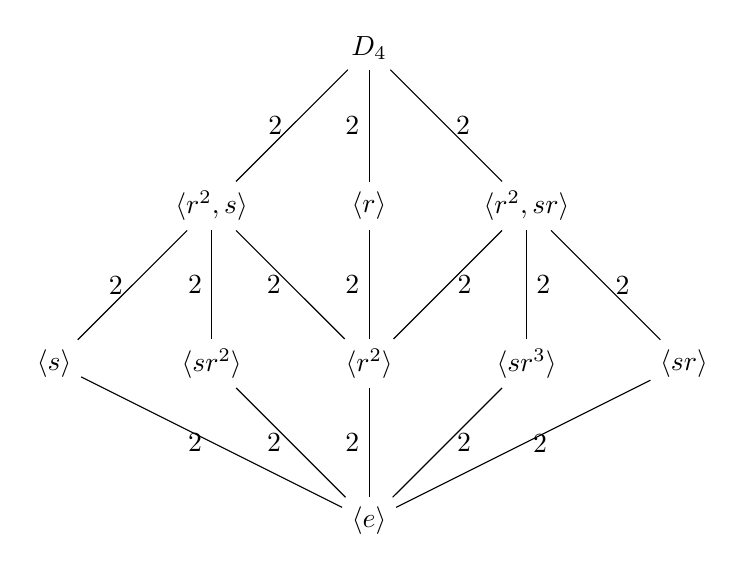
\begin{tikzpicture}[node distance=2cm]
            \node (D4) {$D_4$};
            \node[below of=D4] (r) {$\langle r\rangle$};
            \node[left of=r] (r2s) {$\langle r^2,s\rangle$};
            \node[right of=r] (r2sr) {$\langle r^2,sr\rangle$};
            \node[below of=r] (r2) {$\langle r^2\rangle$};
            \node[left of=r2] (sr2) {$\langle sr^2\rangle$};
            \node[right of=r2] (sr3) {$\langle sr^3\rangle$};
            \node[right of=sr3] (sr) {$\langle sr\rangle$};
            \node[left of=sr2] (s) {$\langle s\rangle$};
            \node[below of=r2] (1) {$\langle e\rangle$};

            \draw (D4) --node[left] {$2$} (r);
            \draw (D4) --node[left] {$2$} (r2s);
            \draw (D4) --node[right] {$2$} (r2sr);
            \draw (r) --node[left] {$2$} (r2);
            \draw (r2s) --node[left] {$2$} (sr2);
            \draw (r2s) --node[left] {$2$} (s);
            \draw (r2s) --node[left] {$2$} (r2);
            \draw (r2sr) --node[right] {$2$} (sr3);
            \draw (r2sr) --node[right] {$2$} (sr);
            \draw (r2sr) --node[right] {$2$} (r2);
            \draw (r2) --node[left] {$2$} (1);
            \draw (sr2) --node[left] {$2$} (1);
            \draw (sr3) --node[right] {$2$} (1);
            \draw (sr) --node[right] {$2$} (1);
            \draw (s) --node[left] {$2$} (1);
        \end{tikzpicture}
        \caption{Diagrama de Hasse para los subgrupos de $D_4$.}
\end{figure}

\noindent
Si dividimos los 5 grupos del centro del diagrama y los dividimos entre $\langle r^2 \rangle $, llegamos a que es isomorfo al grupo de Klein. % // TODO: Hacer precisamente esto
\end{ejemplo}

\subsection{Cuarto Teorema de Isomorfía}
\begin{lema}[Ley modular o regla de Dedekind]
    Sea $G$ un grupo y $A,B,C < G$ con $A<C$, entonces:
    \begin{equation*}
        A(B\cap C) = AB \cap C
    \end{equation*}
    \begin{proof}
        Por doble implicación:
        \begin{description}
            \item [$\subseteq)$] Sea $z\in A(B\cap C)$, entonces existen $a\in A$ y $x\in B\cap C$ de forma que $z=ax$, con lo que:
                \begin{equation*}
                    \left.\begin{array}{r}
                        ax \in AB \\
                        a\in A< C \quad x\in B\cap C \\
                        ax \in AC
                    \end{array}\right\} \Longrightarrow ax\in C \Longrightarrow z\in AB\cap C
                \end{equation*}
            \item [$\supseteq)$] Sea $z\in AB\cap C$, entonces:
                \begin{equation*}
                    \left\{\begin{array}{ll}
                            z = ab, &\quad a\in A, b\in B \\
                            z = c, &\quad c\in C
                    \end{array}\right. 
                \end{equation*}
                Pero por ser $A<C$, tenemos que $a\in C$, con lo que $a^{-1}\in C$, de donde:
                \begin{equation*}
                    b = a^{-1}z \in C
                \end{equation*}
                Pero como $b\in B$, llegamos a que $b\in B\cap C$.
        \end{description}
    \end{proof}
\end{lema}

\begin{observacion}
    Observemos que la hipótesis $A<G$ no es necesaria, pero se obtiene directamente al suponer $A\subseteq G$ y $A<C$ con $C<G$, con lo que no obtenemos más generalidad.
\end{observacion}

\begin{lema}
    Sea $G$ un grupo y $A,B,C<G$ con $B\lhd A$, entonces:
    \begin{enumerate}
        \item[$i)$] $B\cap C\lhd A\cap C$ y $\nicefrac{A\cap C}{B\cap C} \cong \nicefrac{B(A\cap C)}{B}$.
        \item[$ii)$] Si además $C\lhd G$, entonces: $BC\lhd AC$ y $\nicefrac{AC}{BC}\cong \nicefrac{A}{B(A\cap C)}$
    \end{enumerate}

    \begin{figure}[H]
        \centering
        \begin{tikzpicture}
            \node (G) {$G$};
            \node (A) [below =of G] {$A$};
            \node (C) [below =of G, xshift=-1cm] {$C$};
            
            \node (intersec) [below =of A] {$B(A\cap C)$};
            \node (AintersecC) [below left =of intersec] {$A\cap C$};
            \node (B) [below right =of intersec] {$B$};
            \node (res) [below right =of AintersecC] {$B\cap (A\cap C)=B\cap C$};

            \draw (G) -- (A);
            \draw (G) -- (C);
            \draw (A) -- (intersec);
            \draw (A) -- (AintersecC);
            \draw (A) -- (B);
            \draw (C) -- (AintersecC);
            \draw (intersec) -- (B);
            \draw (intersec) -- (AintersecC);
            \draw (AintersecC) -- (res);
            \draw (B) -- (res);
        \end{tikzpicture}
    \end{figure}

    \begin{proof}
        Veamos los dos apartados:
        \begin{enumerate}
            \item[$i)$] Aplicando el Segundo Teorema de Isomorfía sobre el diagrama (observamos el paralelogramo):
                \begin{equation*}
                    \nicefrac{A\cap C}{B\cap C} \cong \nicefrac{B(A\cap C)}{B}
                \end{equation*}
            \item[$ii)$] Ahora, si $C\lhd G$, tenemos que $BC,AC<G$, así como que $BC<AC$ (por ser $B<A$). Para ver que es normal:
                \begin{equation*}
                    \left.\begin{array}{l}
                        x = ac \\
                        x = bc'
                \end{array}\right\} \Longrightarrow xyx^{-1} = acbc'c^{-1}a^{-1} = aca^{-1}aba^{-1}acc'a^{-1} \stackrel{(\ast)}{\in} CBC
                \end{equation*}
                Y si usamos que $C\lhd G$, $B\lhd A$ y $C\lhd G$, llegamos a $(\ast)$:
                \begin{equation*}
                    xyx^{-1} \in CBC = BCC = BC \Longrightarrow BC \lhd AC
                \end{equation*}
                Y como $C\lhd G$, tenemos que $CB = BC$. Ahora, aplicando el Segundo Teorema de Isomorfía sobre el siguiente diagrama:

                \begin{figure}[H]
                    \centering
                    \begin{tikzpicture}
                        \node (HK) {$AC$};
                        \node (H) [below left =of HK] {$A$};
                        \node (K) [below right =of HK] {$BC$};
                        \node (HcapK) [below right =of H] {$BC\cap A = B(A\cap C)$};

                        \draw (G) -- (HK);
                        \draw (HK) -- (H);
                        \draw (HK) -- (K);
                        \draw (H) -- (HcapK);
                        \draw (K) -- (HcapK);
                    \end{tikzpicture}
                \end{figure}
                Llegamos a que:
                \begin{equation*}
                    \nicefrac{A}{B(A\cap C)} \cong \nicefrac{AC}{BC}
                \end{equation*}
        \end{enumerate}
    \end{proof}
\end{lema}

% EL lema anterior se podria hacer tmb para A,B\subseteq G
% Sin embargo, AB solo lo ha definido para subgrupos, no subconjuntos
% SOlo es necesario C < G

% // TODO: Otra clase

A continuación, veremos el Cuarto Teorema de Isomorfía, o Teorema de Zassenhaus, para el cual conviene pensar en la Figura~\ref{fig:4_isomorfia}.

\begin{figure}[H]
    \centering
    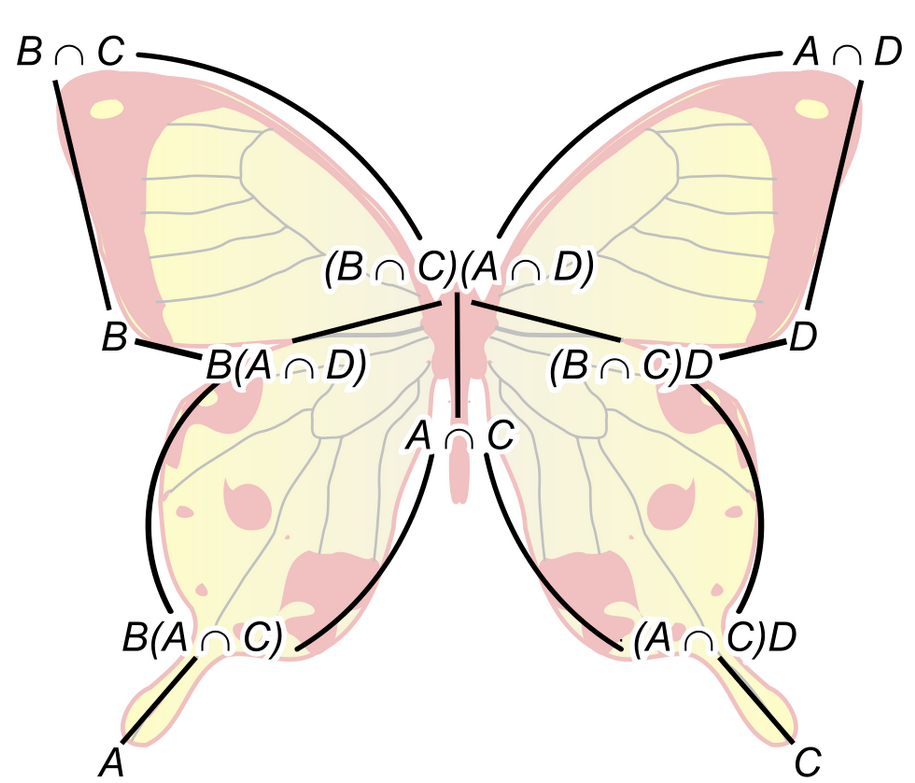
\includegraphics[width=0.8\linewidth]{img/mariposa.png}
    \caption{Situación del Teorema~\ref{teo:4_isomorfia}}
    \label{fig:4_isomorfia}
\end{figure}

% // TODO: NO es necesario aprendérselo
\begin{teo}[Cuarto Teorema de Isomorfía para grupos]\label{teo:4_isomorfia}
    Sea $G$ un grupo y $A_1,C_1,A_2,C_2 < G$ y $C_1\lhd A_1$, $C_2 \lhd A_2$, entonces:
    \begin{enumerate}
        \item[$i)$] $(A_1\cap C_2) C_1 \lhd (A_1 \cap A_2)C_1$.
        \item[$ii)$] $(A_2 \cap C_1) C_2 \lhd (A_1\cap A_2)(C_2)$.
        \item[$iii)$] $\nicefrac{(A_1\cap A_2)C_1}{(A_1\cap C_2)C_1} \cong \nicefrac{A_1\cap A_2}{(A_1\cap C_2)(A_2\cap C_1)}\cong \nicefrac{(A_1\cap A_2)C_2}{(A_2\cap C_1)C_2} $
    \end{enumerate}

    \begin{proof} Veámoslo todo:
        \begin{enumerate}
            \item[$i)$] Si nos fijamos en este retículo, por el Segunto Teorema de Isomorfía tenemos que:
                \begin{figure}[H]
                    \centering
                    \begin{tikzpicture}[node distance=1cm]
                            \node (A2) {$A_2$};

                            \node(A1capC2) [below =of A2] {$A_1\cap C_2$};
                            \node(IntersecA) [below left =of A1capC2] {$A_1\cap A_2$};
                            \node(C2) [below right =of A1capC2] {$C_2$};
                            \node(IntersecC2) [below =of A1capC2, yshift=-1cm] {$(A_1\cap A_2)C_2=A_1\cap C_2$};

                            \draw (A2) -- (A1capC2);
                            \draw (A2) -- (IntersecA);
                            \draw (A2) -- (C2);
                            \draw (A1capC2) -- (IntersecA);
                            \draw (A1capC2) -- (C2);
                            \draw (IntersecA) -- (IntersecC2);
                            \draw (IntersecC2) -- (C2);

                        \end{tikzpicture}
                \end{figure}
                \begin{equation*}
                    \dfrac{A_1\cap A_2}{A_1 \cap C_2} \cong \dfrac{(A_1\cap A_2)C_2}{C_2}
                \end{equation*}
                Así como que $A_1\cap C_2\lhd A_1\cap A_2$. Utilizando el segundo apartado del último Lema, tenemos que:
                \begin{equation*}
                    (A_1\cap C_2)C_1 \lhd (A_1\cap A_2)C_1
                \end{equation*}
            \item[$ii)$] Es análogo.
            \item[$iii)$] Si nos fijamos en, llegamos a que:

                \begin{figure}[H]
                    \centering
                    \shorthandoff{""}
                    \begin{tikzcd}
                                               & A_1 \arrow[ldd, no head] \arrow[d, no head] \arrow[rd, "normal", no head] &     \\
                                               & A_1\cap A_2 \arrow[ld, no head]                                           & C_1 \\
                    (A_1\cap C_2)(C_1\cap A_2) &                                                                           &    
                    \end{tikzcd}    
                    \shorthandon{""}
                \end{figure}


                \begin{equation*}
                    (A_1\cap C_2)(C_1\cap A_2) \lhd A_1\cap A_2
                \end{equation*}
                Ya que teníamos que:
                \begin{gather*}
                    A_1\cap C_2 \lhd A_1\cap A_2 \\
                    C_1\cap A_2 \lhd A_1\cap A_2
                \end{gather*}
                Y:
                \begin{equation*}
                    \dfrac{AC}{BC} = \dfrac{A}{B(A\cap C)}
                \end{equation*}
                Si cogemos:
                \begin{align*}
                    B &= (A_1\cap C_2)(C_1\cap A_2) \\
                    A &= A_1\cap A_2 \\
                    C  &= C_1
                \end{align*}
        \end{enumerate}
    \end{proof}
\end{teo}

\section{Producto directo}
Como vimos en el Capítulo~\ref{cap:1}, dados dos grupos $H$ y $G$, podemos considerar en el conjunto $H\times G$ el grupo directo de estos, \ldots


\begin{definicion}[Producto directo]
    Ya lo vimos en el T1, reescribir.\\

    \noindent
    Distinguiremos entre:
    \begin{itemize}
        \item Producto directo externo (llamado simplemente producto directo y referido a dos grupos cualesquiera).
        \item Producto directo interno (dos subgrupos de un grupo).
    \end{itemize}

    Definimos en el producto cartesiano $(H\times G)\times (H\times G)\to H\times G$ la operación dada por:
    \begin{equation*}
        (h,k)(h_1,k_1) \longmapsto (hh_1, kk_1)
    \end{equation*}
    Que es:
    \begin{itemize}
        \item Asociativa, dada por la asociativa de cada grupo.
        \item Tiene al elemento $(1,1)$ como neutro.
        \item Fijado un elemento $(x,y)\in H\times G$, su elemento inverso será $(x^{-1},y^{-1})$.
    \end{itemize}
    De esta forma, $H\times G$ con dicha operación es un grupo, al que llamaremos grupo directo (externo) de $H$ y $G$.
\end{definicion}

\begin{prop}
    Si $H$ y $K$ son dos grupos finitos, entonces:
    \begin{enumerate}
        \item[$i)$] $|H\times K| = |H||K|$.
        \item[$ii)$] $O(h,k) = \mcm(o(h), o(k))$ $\forall (h,k)\in H\times K$.
    \end{enumerate}
    % \begin{proof} % // TODO: Hacer
    % \end{proof}
\end{prop}

\begin{definicion}[Proyecciones e inyecciones]
    En el producto directo podemos definir 4 aplicaciones que nos serán de utilidad:
    \begin{figure}[H]
        \centering
        \shorthandoff{""}
        \begin{tikzcd}
        H \arrow[r, "i_1", shift left] & H\times G \arrow[r, "p_2"', shift right] \arrow[l, "p_1", shift left] & G \arrow[l, "i_2"', shift right]
        \end{tikzcd}    
        \shorthandon{""}
    \end{figure}

    \begin{align*}
        i_1(h) &= (h,1) \\
        i_2(k) &= (1,k) \\
        p_1(h,k) &= h \\
        p_2(h,k) &= k
    \end{align*}
    A $i_1$ y $i_2$ las llamaremos inyecciones y a $p_1$ y $p_2$ las llamaremos proyecciones.
\end{definicion}

\begin{prop}
    Se verifica que:
    \begin{enumerate}
        \item $p_j$ y $i_j$ con $j\in \{1,2\}$ son homomorfismos de grupos.
        \item $p_ji_j = id$, y si $p_ji_k$ con $i\neq k$, es trivial.
        \item $p_j$ son sobreyectivas y $i_j$ son inyectivas.
        \item Se tiene que:
            \begin{equation*}
                H' = Im(i_1) = \ker(p_2) = \{(h,1) \mid h\in H\} \lhd H\times G
            \end{equation*}
            Además, $H'\cong H$.
        \item De la misma forma:
            \begin{equation*}
                G' = Im(i_2) = \ker(p_1) = \{(1,k)\mid k\in G\} \lhd H\times G
            \end{equation*}
            Además, $G'\cong G$.
        \item $H'\cap G' = \{1\}$.
        \item $xy = yx$ para todo $x\in H'$, $y\in G'$.
    \end{enumerate}
    % \begin{proof} % // TODO: HACER
    % \end{proof}
\end{prop}

\subsection{Caracterización del grupo directo por isomorfismo}

\begin{teo}[Propiedad universal del producto directo]\label{teo:prop_universal_directo}
    Sea $G$ un grupo y $f_1:G\to H$, $f_2:G\to K$ dos homomorfismos de grupos, entonces existe un único homomorfismo de grupos $f:G\to H\times K$ tal que $p_1f=f_1$ y $p_2f = f_2$

    \begin{figure}[H]
        \centering
        \shorthandoff{""}
        \begin{tikzcd}
          & G \arrow[ld, "f_1"] \arrow[rd, "f_2"] \arrow[d, "f", dashed] &   \\
        H & H\times K \arrow[l, "p_1"] \arrow[r, "p_2"]                  & K
        \end{tikzcd}
        \shorthandon{""}
    \end{figure}

    \begin{proof}
        Definimos $f:G\to H\times K$ dada por:
        \begin{equation*}
            f(g) = (f_1(g), f_2(g)) \qquad \forall g\in G
        \end{equation*} % // TODO: Terminar
    \end{proof}
\end{teo}

El producto directo es único salvo isomorfismos. Es decir, que si hay otro grupo que verifica la propiedad universal de grupo directo, este debe ser isomorfo al grupo directo.
\begin{teo}
   Sea $L$  un grupo y $l_1:L\to H$, $l_2:L\to K$ dos homomorfismos de grupos que verifican para todo grupo $G$ y para todo par de homomorfismos $f_1:G\to H$ y $f_2:G\to K$ existe un único homomorfismo $f:G\to L$ tal que si $l_1f = f_1$ y $l_2f = f_2$, entonces:
   \begin{equation*}
       L \cong H\times K
   \end{equation*}


   \begin{figure}[H]
       \centering
       \shorthandoff{""}
        \begin{tikzcd}
          & L \arrow[rd, "h_2"] \arrow[ld, "h_1"]                         &   \\
        H &                                                               & K \\
          & G \arrow[lu, "f_1"] \arrow[ru, "f_2"] \arrow[uu, "f", dashed] &  
        \end{tikzcd}
       \shorthandon{""}
   \end{figure}

   \begin{proof}
       Por el Teorema anterior y observando que:
       \begin{figure}[H]
           \centering
           \shorthandoff{""}
            \begin{tikzcd}
              & L \arrow[rd, "l_2"] \arrow[ld, "l_1"] \arrow[d, "f", dashed] &   \\
            H & H\times K \arrow[r, "p_2"] \arrow[l, "p_1"]                  & K
            \end{tikzcd}
           \shorthandon{""}
       \end{figure}
       Tenemos que $p_2l = l_1$ y que $p_1l = l_1$. Ahora:
       \begin{equation*}
           p_1 1_{H\times K} = p_1 =  l_1 p = p_1 l p \Longrightarrow lp = 1_{H\times K}
       \end{equation*}
       \begin{equation*}
           l_1 1_G = l_1 = p_1l = l_1pl \Longrightarrow 1_G = pl
       \end{equation*}
   \end{proof}
\end{teo}

Y lo mismo que hemos hecho para las proyecciones se puede hacer para las inyecciones:

\begin{teo}\label{teo:prop_universal_directo}
    Sea $G$ un grupo y $f_1:H\to G$, $f_2:K\to G$ dos homomorfismos de grupos, entonces existe un único homomorfismo de grupos $f:H\times K\to G$ tal que $fi_1 = f_1$, $fi_2 = f_2$.

    \begin{figure}[H]
        \centering
        \shorthandoff{""}
            \begin{tikzcd}
                                                   & G                                 &                                        \\
            H \arrow[ru, "f_1"'] \arrow[r, "i_1"'] & H\times K \arrow[u, "f"', dashed] & K \arrow[lu, "f_2"'] \arrow[l, "i_2"']
            \end{tikzcd}
        \shorthandon{""}
    \end{figure}

    \begin{proof}
        Ahora, definiremos:
        \begin{equation*}
            f(h,k) = f_1(h)f_2(k)
        \end{equation*}
        Con lo que tendremos:
        \begin{equation*}
            f((h,1)(1,k)) = f(h,k) = f_1(h)f_2(k) = f_1(h,k) f_2(h,k)
        \end{equation*}
    \end{proof}
\end{teo}

\begin{teo}
   Sea $L$  un grupo y $l_1:H\to L$, $l_2:K\to L$ dos homomorfismos de grupos que verifican que
   \begin{equation*}
       l_1(h)l_2(k) = l_2(k)l_1(h) \qquad \forall h\in H, k\in K
   \end{equation*}
   y que para todo grupo $G$ y para todo par de homomorfismos $f_1:G\to H$ y $f_2:G\to K$ tales que
   \begin{equation*}
       f_1(h)f_2(k) = f_2(k)f_1(h) \qquad \forall h\in H, k\in K
   \end{equation*}
   existe un único homomorfismo $f:L\to G$ tal que si $fl_1 = f_1$ y $fl_2 = f_2$, entonces:
   \begin{equation*}
       L \cong H\times K
   \end{equation*}

   % // TODO: Cambiar diagrama
   % \begin{figure}[H]
   %     \centering
   %     \shorthandoff{""}
   %      \begin{tikzcd}
   %        & L \arrow[rd, "h_2"] \arrow[ld, "h_1"]                         &   \\
   %      H &                                                               & K \\
   %        & G \arrow[lu, "f_1"] \arrow[ru, "f_2"] \arrow[uu, "f", dashed] &  
   %      \end{tikzcd}
   %     \shorthandon{""}
   % \end{figure}

   \begin{proof}
   \end{proof}
\end{teo}

% Copiar para familia de grupos

\section{Producto directo interno}
Qué sucede cuando $H,K<G$ y caracterizar cuando $H\times K \cong G$.
